\documentclass[conference]{IEEEtran}
\usepackage{cite}
\usepackage{amsmath,amssymb,amsfonts}
\usepackage{graphicx}
\usepackage{textcomp}
\usepackage{xcolor}
\usepackage[hidelinks]{hyperref}
\usepackage{booktabs}
\usepackage{listings}
\usepackage{array}
\usepackage{enumitem}
\usepackage{url}
\graphicspath{{./}}

\setlist[itemize]{leftmargin=*, topsep=2pt, itemsep=2pt, parsep=0pt}
\setlist[enumerate]{leftmargin=*, topsep=2pt, itemsep=2pt, parsep=0pt}

\def\BibTeX{{\rm B\kern-.05em{\sc i\kern-.025em b}\kern-.08em
    T\kern-.1667em\lower.7ex\hbox{E}\kern-.125emX}}

\lstset{
  basicstyle=\ttfamily\scriptsize,
  breaklines=true,
  frame=single,
  framesep=3pt,
  xleftmargin=6pt,
  xrightmargin=6pt,
  aboveskip=4pt,
  belowskip=4pt,
  captionpos=t,
  numbers=none,
  tabsize=2
}

\begin{document}

\title{Roameo: An Agentic Approach to Automated Travel Itinerary Optimization}

\author{
\begin{tabular}{cc}
\multicolumn{2}{c}{
\begin{minipage}{0.45\linewidth}
\centering
\textbf{Mrs. V. Savitri}\\
Sr. Assistant Professor\\
Vignan's Institute of Information Technology\\
Visakhapatnam, India
\end{minipage}
} \\[3em]

\begin{minipage}{0.45\linewidth}
\centering
\textbf{Desireddy Venkata Mahendra Reddy}\\
Department of CSE (AI)\\
Vignan's Institute of Information Technology\\
Visakhapatnam, India
\end{minipage}
&
\begin{minipage}{0.45\linewidth}
\centering
\textbf{Kuramdasu Yaswanth}\\
Department of CSE (AI)\\
Vignan's Institute of Information Technology\\
Visakhapatnam, India
\end{minipage}
\\[3em]
\begin{minipage}{0.45\linewidth}
\centering
\textbf{Mayank Yadav}\\
Department of CSE (AI)\\
Vignan's Institute of Information Technology\\
Visakhapatnam, India
\end{minipage}
&
\begin{minipage}{0.45\linewidth}
\centering
\textbf{Polumati Ryan Ike}\\
Department of CSE (AI)\\
Vignan's Institute of Information Technology\\
Visakhapatnam, India
\end{minipage}
\end{tabular}
}

\maketitle

\begin{abstract}
Travel planning remains fragmented across maps, reviews, weather pages, booking searches, and conversational assistants. Many recent systems respond with fluent text but still leave itinerary consistency, route feasibility, and state persistence unresolved. This paper presents \textit{Roameo}, a conversational travel-planning workspace built around a router-first runtime, deterministic tool execution, and one canonical session snapshot shared across chat, itinerary, map, and saved places. The current system uses a lightweight fast path for trivial turns, a semantic intent resolver for travel understanding, direct grounding through Google Places and related travel APIs, structured itinerary synthesis for planning turns, deterministic feasibility and transit passes, and final narrative generation over the updated canonical state. The implementation combines a Next.js frontend, an Express backend, authenticated Server-Sent Events for live updates, and Supabase-backed persistence. Unlike the earlier project architecture, the current design does not rely on a monolithic travel agent or parallel truth systems. Instead, it separates semantic understanding from deterministic mutations and commits all important artifacts through session-scoped persistence. The result is a practical full-stack architecture for travel planning in which route logic, place discovery, and conversational responses remain synchronized across multiple turns.
\end{abstract}

\begin{IEEEkeywords}
Conversational AI, Travel Planning, Session Snapshot, Multi-Agent Runtime, Router-First Architecture, Server-Sent Events, Google Places API, Supabase, Deterministic Tooling.
\end{IEEEkeywords}

\section{Introduction}

Modern trip planning is still a high-friction activity despite the abundance of digital travel tools. A traveler may use one application to find attractions, another to estimate travel times, a third to check weather conditions, and a fourth to organize the final itinerary. The burden of combining those sources usually falls back on the user. The practical problem is therefore not only retrieval of information, but also coordination of multiple travel facts into one coherent plan.

Large language models have improved the quality of natural-language interaction, but a fluent response alone does not solve the planning problem. A model can describe a trip convincingly while still inventing places, ignoring travel-time constraints, or losing track of earlier user preferences. Prior work on transformer models \cite{vaswani2017attention,brown2020language} and instruction alignment \cite{ouyang2022training} explains why modern systems are capable of handling open-ended travel requests, but production travel planning requires more than text generation. It requires grounded retrieval, explicit state management, and deterministic repair of inconsistent outputs.

Recent agentic techniques such as Reflexion \cite{shinn2023reflexion}, ReAct \cite{yao2023react}, and graph-based orchestration frameworks \cite{langchain2022,langgraph2024} suggest a more reliable direction. The common idea is to decompose complex tasks into narrower stages, allow tools to provide real-world evidence, and maintain an explicit working state instead of relying on one oversized prompt. In recommender settings, structured grounding and explainability have also become more important \cite{zheng2023chatrec,koren2009matrix}.

Roameo follows that direction, but the current implementation differs substantially from the older architecture previously documented in this project. The canonical runtime is now \textit{session-snapshot based}: the same persisted session state drives chat, itinerary, map projection, and saved POIs. The system is also \textit{router first}: conversational short-circuiting handles trivial turns, a semantic resolver handles travel intent, and deterministic services execute grounding and state mutation before the final narrative is generated. Streaming is delivered through Server-Sent Events rather than the older WebSocket-centric design. These changes make the system easier to debug, easier to persist safely, and less likely to drift into parallel or conflicting views of the same trip.

This paper rewrites the project description around the current architecture rather than the superseded one. It focuses on the present router-first planning runtime, the session repository model, the travel-tool grounding layer, and the synchronized frontend surface. The objective is not to present Roameo as a generic AI travel chatbot, but as a concrete full-stack design pattern for reliable conversational planning.

\section{Related Work}

\subsection{Large Language Models for Structured User Intent}

The transformer architecture established the modern foundation for sequence modeling and contextual language understanding \cite{vaswani2017attention}. Subsequent large-scale language models showed that broad generalization can emerge from scale alone \cite{brown2020language}, while instruction tuning and feedback-driven alignment made these models better suited for user-facing systems \cite{ouyang2022training}. In practice, these developments allow a system such as Roameo to interpret open-ended requests like ``plan a relaxed three-day trip with seafood and beach time'' without forcing the user into a rigid form.

\subsection{Reasoning-and-Acting Agent Patterns}

ReAct demonstrated that reasoning traces and tool actions can be interleaved rather than treated as separate workflows \cite{yao2023react}. Reflexion pushed this further by showing that iterative self-correction can improve task outcomes \cite{shinn2023reflexion}. These ideas are useful for travel planning because itineraries frequently need repair after initial synthesis: over-packed days, missing stay assignments, or unrealistic transfers are not rare edge cases but common outcomes of open-ended planning.

\subsection{Graph and Stateful Orchestration}

Application frameworks such as LangChain popularized the decomposition of complex LLM tasks into chains and tools \cite{langchain2022}. More recent graph-oriented orchestration systems formalized shared state and conditional stage transitions as first-class design elements \cite{langgraph2024}. Roameo adopts the stateful orchestration idea, but in the current implementation the shared state is not a framework-owned graph state alone; it is a canonical session snapshot that must remain valid across persistence, streaming, and UI rendering.

\subsection{Recommendation and Planning Grounding}

Knowledge-grounded recommendation research has emphasized the importance of linking natural-language generation to explicit evidence \cite{zheng2023chatrec}. In travel systems, collaborative filtering remains useful for ranking and preference inference \cite{koren2009matrix}, but it does not guarantee factual correctness of destination-specific content. Roameo therefore treats external travel APIs, especially Google Places, as the canonical source of POI truth, while LLMs are used for interpretation, synthesis, and explanation rather than fabricating the catalog.

\subsection{Operational and Interface Considerations}

Usability research remains relevant because planning is a latency-sensitive and cognitively loaded task \cite{nielsen1993usability}. Likewise, system-level concerns such as connection overhead in database-backed applications materially affect user experience \cite{nance2011connection}. These concerns are not peripheral in Roameo; they shape the design choices of session persistence, selective mutation, and streaming delivery.

\section{Problem Definition}

Roameo addresses a practical systems problem: how to transform a free-form travel request into a coherent, persistent, and reviewable planning workspace without splitting state across independent subsystems. The challenge is not only to answer questions, but to maintain agreement between four user-visible artifacts:

\begin{itemize}
  \item the conversational explanation of the trip,
  \item the structured itinerary,
  \item the map view and route overlays,
  \item the saved catalog of relevant places.
\end{itemize}

In many conversational systems these artifacts emerge from partially independent logic paths. A chat response may reflect a newer interpretation than the itinerary, or the map may be based on stale places while the saved list reflects a different search. Roameo explicitly treats such divergence as a design failure. The system therefore enforces a single canonical session snapshot that all these views derive from.

Formally, the input to the system at turn $t$ is the pair $(m_t, s_t)$, where $m_t$ is the current user message and $s_t$ is the session snapshot before processing. The output is an updated snapshot $s_{t+1}$ plus a narrative response derived from that updated state. The architecture is designed so that semantic interpretation may use a model, but state mutation, catalog persistence, route enrichment, and final commit remain explicit and inspectable.

\section{Current System Architecture}

\subsection{Architectural Overview}

The current Roameo architecture has four major layers:

\begin{enumerate}
  \item \textbf{Frontend workspace layer}: a Next.js interface that renders chat, itinerary, map, and saved places from the same session snapshot.
  \item \textbf{API and streaming layer}: an Express backend with authenticated request handling and Server-Sent Events for live session updates.
  \item \textbf{Planning runtime layer}: a router-first turn runner that coordinates semantic resolution, grounding, synthesis, deterministic critique, and final response generation.
  \item \textbf{Persistence layer}: a Supabase-backed repository that stores travel sessions, messages, plan snapshots, POI catalogs, and saved POIs.
\end{enumerate}

This architecture replaces the old description of Roameo as a LangGraph-driven, nine-agent, WebSocket-first system. The current codebase still contains specialized planning stages, but most of them are plain TypeScript functions coordinated by the turn runner rather than independent, freeform agents. This distinction matters because the goal of the modernized runtime is not to maximize agent autonomy; it is to maximize consistency of state and predictability of behavior.

\begin{figure}[htbp]
\centering
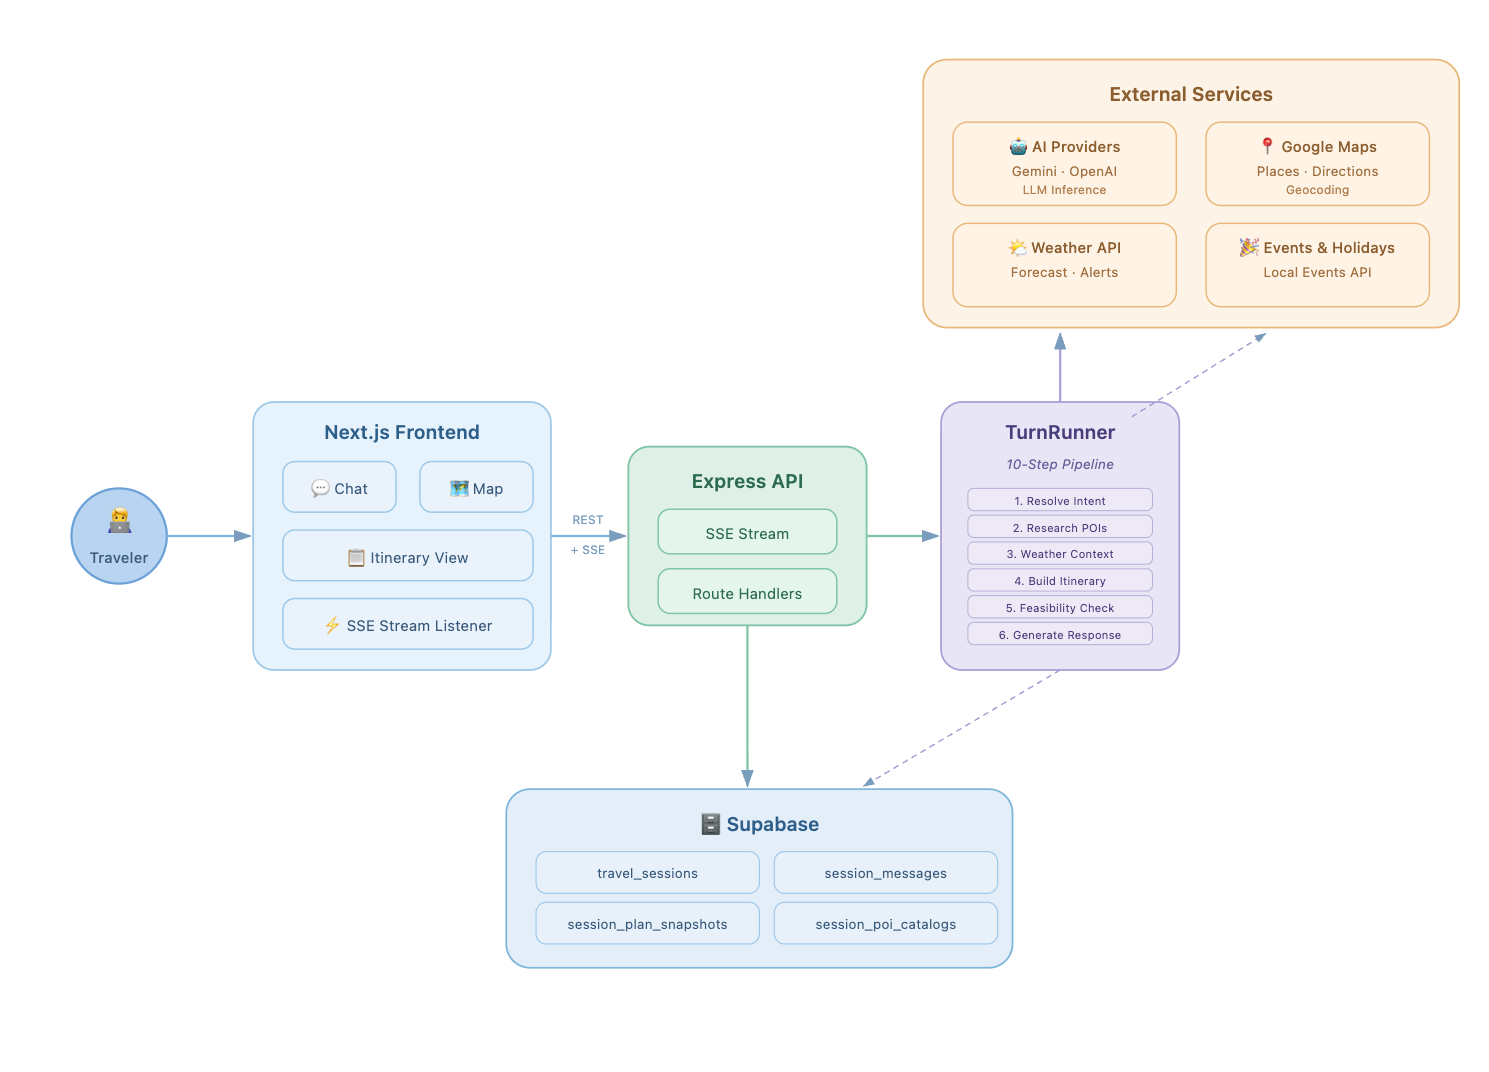
\includegraphics[width=0.48\textwidth]{architecture.png}
\caption{Current Roameo architecture showing the text-first frontend, Express API with SSE, router-first turn runner, Supabase persistence, and external travel services.}
\label{fig:roameo-architecture}
\end{figure}

\begin{table}[htbp]
\caption{Current Roameo Architecture by Layer}
\label{tab:layers}
\centering
\begin{tabular}{p{2.2cm} p{5.3cm}}
\toprule
\textbf{Layer} & \textbf{Primary Responsibility} \\
\midrule
Frontend workspace & Render chat, itinerary, map, and saved places from one session view \\
API + streaming & Accept requests, stream updates, and expose canonical session events \\
Planning runtime & Resolve intent, ground travel facts, synthesize plans, repair feasibility, and narrate results \\
Persistence & Store sessions, messages, plan versions, POI catalogs, and saved POIs \\
\bottomrule
\end{tabular}
\end{table}

\subsection{Canonical Session Snapshot}

The session snapshot is the center of the architecture. It contains provider settings, memory, messages, the current plan when present, the POI catalog, and saved POI identifiers. A simplified view is shown below.

\begin{lstlisting}[language={}, caption={Simplified canonical session snapshot}]
{
  "id": "session-id",
  "title": "Goa, 3 days",
  "providerSettings": { ... },
  "memory": { ... },
  "plan": { ... },
  "poiCatalog": { "version": 1, "items": { ... } },
  "messages": [ ... ],
  "savedPoiIds": [ ... ]
}
\end{lstlisting}

This structure allows chat, itinerary, map, and saved places to be different projections of the same persisted state. It also allows the runtime to reload the session after mutations and generate the final response from the canonical post-tool state rather than from stale intermediate data.

\subsection{Design Invariants}

The current implementation is organized around a small set of invariants:

\begin{itemize}
  \item chat, itinerary, map, and saved POIs must derive from the same session snapshot,
  \item explicit new-trip requests must replace stale active-trip context,
  \item multi-city trips must preserve the destination set instead of collapsing to one city,
  \item discovery POIs may accumulate in the session catalog across turns,
  \item itinerary-linked routes should change only when the canonical plan changes.
\end{itemize}

These invariants are important because they constrain the planning runtime to behave like a stateful system rather than a sequence of unrelated model responses.

\subsection{Session Repository and Persistence Model}

The session repository creates, reads, and updates the canonical session while also separating supporting tables by concern. The current implementation persists session headers in \texttt{travel\_sessions}, conversation turns in \texttt{session\_messages}, plan versions in \texttt{session\_plan\_snapshots}, catalogs in \texttt{session\_poi\_catalogs}, and saved places in \texttt{session\_saved\_pois}. This split supports versioned plans and avoids overloading a single row with every runtime artifact.

The repository also supports a memory-backed fallback for non-Supabase environments, but the canonical production lane is session persistence through Supabase with schema validation on the TypeScript side. This is important because Roameo is not a stateless demo; long-lived planning and follow-up questions depend on session continuity.

\subsection{Streaming Model}

The current runtime emits streaming events through a stream hub and exposes them through Server-Sent Events. This is a substantial architectural change from the older paper draft that centered the system around WebSockets. SSE is sufficient for the one-way, server-to-client event stream Roameo needs:

\begin{itemize}
  \item message deltas while the assistant response is being assembled,
  \item committed message notifications,
  \item plan updates,
  \item session snapshot refreshes,
  \item turn lifecycle events.
\end{itemize}

Because the client ultimately rebuilds from session snapshots, SSE fits the new architecture better than a custom bidirectional socket protocol.

\section{Router-First Planning Runtime}

\subsection{Turn Lifecycle}

The current turn runner executes a deterministic sequence. The user message is persisted first, then the system evaluates whether the turn can be handled by a lightweight conversational fast path. If not, the runtime resolves intent, determines whether discovery and enrichment are needed, optionally synthesizes or refines a plan, performs deterministic post-processing, generates the final narrative, and finally commits the updated session state.

At a high level, the current per-turn pipeline is:

\begin{enumerate}
  \item Persist the user message.
  \item Short-circuit trivial conversational turns.
  \item Resolve travel intent and semantic focus.
  \item Decide whether discovery and research are required.
  \item Retrieve places and supporting travel context.
  \item Synthesize or refine a structured plan when the turn is planning-oriented.
  \item Run deterministic feasibility and transit passes.
  \item Generate the final assistant narrative and structured response blocks.
  \item Derive next follow-up context and update session memory.
  \item Commit the final snapshot with planning state marked \texttt{ready}.
\end{enumerate}

This flow is designed so that every successful turn ends with \texttt{planningState.status = "ready"}, which the frontend uses as an animation and synchronization gate.

\begin{table}[htbp]
\caption{Deterministic Turn Pipeline}
\label{tab:turnpipeline}
\centering
\begin{tabular}{p{0.65cm} p{6.9cm}}
\toprule
\textbf{Step} & \textbf{Operation} \\
\midrule
1 & Persist the user message and emit a committed-message event \\
2 & Check the lightweight conversational fast path \\
3 & Resolve travel intent and semantic focus \\
4 & Decide whether discovery or research is required \\
5 & Retrieve places and date-sensitive travel context \\
6 & Synthesize or refine a structured plan \\
7 & Enrich logistics and run feasibility and transit passes \\
8 & Generate the final narrative and structured response blocks \\
9 & Update follow-up context and session memory \\
10 & Persist the final snapshot and mark planning state as ready \\
\bottomrule
\end{tabular}
\end{table}

\subsection{Fast Path and Semantic Routing}

Not every incoming message deserves a heavy planning pass. The function \texttt{resolveFastTurnResponse()} handles greetings, acknowledgements, identity questions, and similar low-risk turns directly. More substantive travel messages go through \texttt{resolveTurnIntent()}, which extracts destination scope, total days, traveler count, style cues, date context, follow-up ambiguity, and other structured fields from the message and session state.

This router-first design reduces unnecessary tool execution while preserving a consistent interface. It also clarifies the role of the LLM in the pipeline: the model is used where semantic interpretation is genuinely needed, not as a universal replacement for tool planning or state mutation.

\subsection{Current Provider Routing}

The backend supports both Gemini and OpenAI as first-class providers, but the runtime does not treat all planning subtasks as equivalent. Understanding and routing favor fast models, while synthesis and narrative generation use models better suited to structured travel responses. This split reflects a practical engineering judgment: classification, tool planning, and user-facing explanation do not share the same latency or quality profile, and therefore should not be forced through one universal model choice.

\subsection{Research and Grounding}

Roameo grounds travel knowledge through explicit services rather than generated guesses. The current tool layer uses the Google Places API as the canonical POI source \cite{googleplaces2024} together with supporting travel services:

\begin{itemize}
  \item Google Places for POI retrieval,
  \item Google Geocoding for destination resolution,
  \item Google Directions for route estimates,
  \item Open-Meteo for weather summaries,
  \item Tavily for broader destination and event research when enabled,
  \item Nager.Date for holiday context.
\end{itemize}

An important engineering rule in the current codebase is that every Google Places text search applies a type filter. Stays, restaurants, and attractions are mapped to the corresponding Places types so that restaurant queries do not leak viewpoints and attraction queries do not contaminate accommodation results. This explicit type filtering is a small implementation detail with large UX consequences because category bleed quickly erodes trust in a planning system.

\subsection{Structured Plan Synthesis}

For \texttt{plan\_trip} and \texttt{refine\_trip} turns, the runtime calls \texttt{synthesizePlan()} with the resolved intent and grounded research. The synthesis stage does not own the entire correctness burden. After initial plan generation, the runtime enriches logistics, assigns stays where needed, repairs hospitality gaps, and then passes the result through a deterministic feasibility critic.

This post-processing step is deliberate. In open-ended planning, the first generated structure is often directionally useful but operationally imperfect. By separating synthesis from repair, Roameo avoids the fragile pattern in which a single prompt is expected to understand user intent, choose places, check routing, verify accommodation logic, and narrate the result without code-level safeguards.

\subsection{Feasibility Critic and Transit Advisor}

Two specialized deterministic passes follow synthesis:

\begin{itemize}
  \item \textbf{Feasibility critic}: trims over-packed days, flags unrealistic transfers, and repairs missing accommodation or route assumptions.
  \item \textbf{Transit advisor}: evaluates inter-destination transit segments, especially for multi-destination plans.
\end{itemize}

These passes reflect the project's move away from ``everything in one generation'' toward narrower, auditable responsibilities. They also make the system's internal behavior easier to surface to the user via streamed progress labels and trace-like updates.

\subsection{Narrative Generation Over Updated State}

Only after the grounded and repaired state is available does Roameo call \texttt{answerConversationally()}. This ordering is a core architectural choice. The assistant does not narrate an intended plan and then hope persistence catches up later. Instead, the message is generated from the updated session and then emitted in chunks to the frontend. The final committed assistant message stores response blocks and follow-up context in its metadata, which lets the UI remain synchronized with what the model actually said.

\subsection{Canonical Mutation Surface}

Another important property of the current architecture is that session-aware changes are intended to pass through a narrow mutation surface rather than arbitrary business logic scattered across the application. The broader project direction includes explicit tool-style mutation primitives for actions such as trip-header updates, itinerary edits, memory updates, active-trip resets, and follow-up persistence. Even when the turn runner performs direct repository writes in the current implementation, the architectural principle remains the same: canonical session state should be changed through centralized, inspectable mutation paths rather than through hidden frontend-only or prompt-only state.

\section{Implementation Details}

\subsection{Frontend Surface}

The frontend is a text-first workspace built in Next.js. The left side centers the conversation, while the right side presents itinerary or map views as structured projections of the current session. This division matters because Roameo is not a single chat transcript with incidental maps; it is a coordinated planning workspace where conversational input, route understanding, and itinerary structure must remain aligned.

The client consumes authenticated SSE events and updates local stores from canonical session snapshots. This eliminates a class of synchronization bugs in which the client tries to reconstruct truth from partial response fragments. The design also makes the system more resilient to refreshes and multi-turn refinement because the snapshot, not the transient UI state, is authoritative.

\begin{figure}[htbp]
\centering
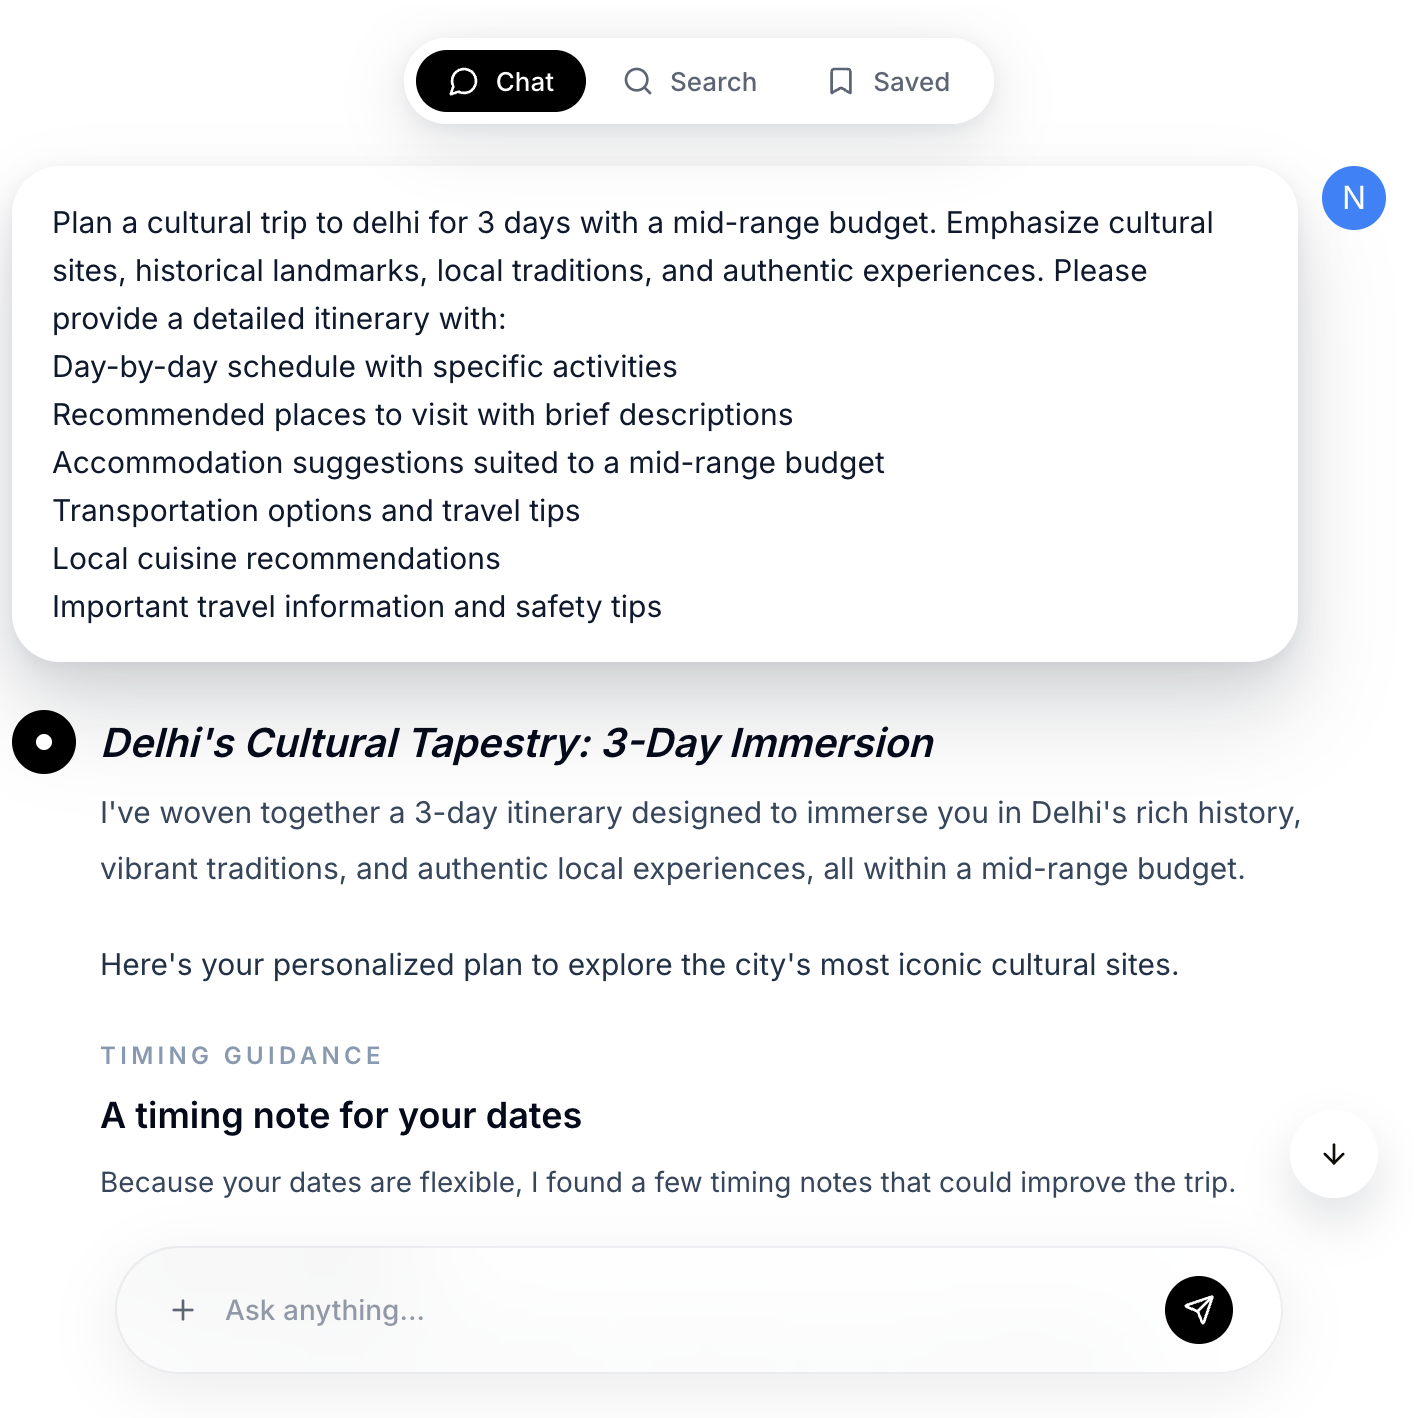
\includegraphics[width=0.46\textwidth]{05_chat.png}
\caption{Roameo's text-first planning workspace. The assistant response is grounded into structured planning output while the frontend remains synchronized through canonical session updates.}
\label{fig:roameo-chat}
\end{figure}

\subsection{Backend Services}

The backend is implemented in TypeScript on Express. The turn runner coordinates the planning workflow, the travel-tools service handles grounded retrieval and enrichment, and the session repository centralizes persistence. This separation of concerns keeps the planning path understandable:

\begin{itemize}
  \item \texttt{turn-runner.ts} owns turn sequencing and stream emission,
  \item \texttt{subagents.ts} owns semantic resolution, synthesis, and narrative functions,
  \item \texttt{travel-tools.ts} owns geocoding, Places search, weather, events, and holiday lookup,
  \item \texttt{session-repository.ts} owns session, message, plan, and catalog persistence.
\end{itemize}

The result is a codebase in which travel intelligence is not hidden inside one very long prompt or one oversized controller. Each stage has a narrow purpose and an obvious failure surface.

\subsection{Provider Model}

The canonical project direction treats both Gemini and OpenAI as first-class providers. Provider defaults and key-source settings are stored in user/session settings rather than hardcoded into the UI. The runtime resolves providers through a shared provider service, and the turn runner carries those settings through message commit, synthesis, and final response generation.

This design matters for two reasons. First, it prevents provider selection from becoming a hidden source of behavioral divergence. Second, it allows the same session model to support both platform-managed and bring-your-own-key usage without splitting business logic.

\section{Evaluation Perspective}

The rewritten paper does not claim old performance numbers inherited from the superseded architecture. Instead, the current implementation supports a more defensible evaluation framing based on four dimensions:

\begin{enumerate}
  \item intent and routing quality,
  \item factual grounding of discovered places,
  \item consistency across chat, itinerary, and map projections,
  \item responsiveness of the streamed planning experience.
\end{enumerate}

The project repository and associated college documentation already include benchmark tables, intent-evaluation discussions, interface walkthrough material, and load-testing workflows built around Artillery \cite{artillery2024}. In the context of this paper, the most important engineering takeaway is that quality is not determined only by one model response. It depends on whether the runtime commits one consistent session state and whether user-visible panels reflect that state without divergence.

\section{Limitations and Future Work}

Despite the architectural improvements, the current system still has limitations. Preference memory remains primarily session-scoped rather than truly cross-session and user-global. Richer booking integration is not yet part of the canonical runtime. Some destination research remains dependent on optional external services and therefore inherits the availability and quality of those providers. The frontend workspace is also strongest for desktop-style use; more work is needed to make the same planning density feel natural on smaller screens.

Future work can extend the current architecture without abandoning its core principles. The most valuable extensions are likely to be:

\begin{itemize}
  \item live booking integrations for flights, stays, and activities,
  \item stronger long-term preference memory beyond one session,
  \item improved explanation surfaces for why each POI or route was chosen,
  \item multilingual planning support,
  \item richer shared or collaborative planning sessions.
\end{itemize}

The important constraint is that these additions should continue to route through the canonical session state rather than introducing parallel truth systems.

\section{Conclusion}

Roameo is best understood not as a generic AI trip planner, but as a concrete architecture for reliable conversational planning. The current system moves away from the earlier monolithic, loosely synchronized design and toward a router-first runtime in which semantic interpretation, grounded retrieval, deterministic repair, narrative generation, and state persistence are clearly separated. Its most important idea is simple but powerful: chat, itinerary, map, and saved places should all derive from one canonical session snapshot.

That design choice affects every layer of the implementation. It changes how messages are persisted, how stream events are emitted, how plans are repaired after generation, how UI panels are synchronized, and how follow-up turns inherit context. By embedding LLM reasoning inside a deterministic, tool-grounded, session-scoped runtime, Roameo demonstrates a practical full-stack pattern for conversational travel planning that is more robust than both plain chatbot interfaces and old-style siloed travel apps.

\begin{thebibliography}{00}

\bibitem{vaswani2017attention}
A.~Vaswani, N.~Shazeer, N.~Parmar, J.~Uszkoreit, L.~Jones, A.~N.~Gomez,
\L.~Kaiser, and I.~Polosukhin, ``Attention is all you need,''
\textit{Advances in Neural Information Processing Systems}, vol.~30, pp.~5998--6008, 2017.

\bibitem{brown2020language}
T.~Brown, B.~Mann, N.~Ryder, M.~Subbiah, J.~D.~Kaplan, P.~Dhariwal, et al.,
``Language models are few-shot learners,''
\textit{Advances in Neural Information Processing Systems}, vol.~33, pp.~1877--1901, 2020.

\bibitem{ouyang2022training}
L.~Ouyang, J.~Wu, X.~Jiang, D.~Almeida, C.~Wainwright, P.~Mishkin, et al.,
``Training language models to follow instructions with human feedback,''
\textit{Advances in Neural Information Processing Systems}, vol.~35, 2022.

\bibitem{shinn2023reflexion}
N.~Shinn, F.~Cassano, B.~Labash, A.~Gopinath, K.~Narasimhan, and S.~Yao,
``Reflexion: Language agents with verbal reinforcement learning,''
\textit{Advances in Neural Information Processing Systems}, vol.~36, 2023.

\bibitem{yao2023react}
S.~Yao, J.~Zhao, D.~Yu, N.~Du, I.~Shafran, K.~Narasimhan, and Y.~Cao,
``ReAct: Synergising reasoning and acting in language models,''
in \textit{Proceedings of ICLR 2023}, 2023.

\bibitem{langchain2022}
H.~Chase, ``LangChain: Building applications with large language models,''
\textit{GitHub Repository}. [Online]. Available: \url{https://github.com/langchain-ai/langchain}

\bibitem{zheng2023chatrec}
Y.~Zheng, R.~Zhang, J.~Zhang, Y.~Ye, Z.~Luo, Z.~Feng, and Y.~Ma,
``ChatRec: Towards interactive and explainable LLMs-augmented recommender system,''
\textit{arXiv preprint arXiv:2303.14524}, 2023.

\bibitem{koren2009matrix}
Y.~Koren, R.~Bell, and C.~Volinsky,
``Matrix factorization techniques for recommender systems,''
\textit{Computer}, vol.~42, no.~8, pp.~30--37, 2009.

\bibitem{nielsen1993usability}
J.~Nielsen, \textit{Usability Engineering}. Academic Press, 1993.

\bibitem{nance2011connection}
D.~Nance and K.~Hazelwood,
``Connection pool overhead in database-backed web applications,''
in \textit{Proceedings of the 2011 MobiSys Workshop on Mobile Cloud Computing \& Services}, 2011.

\bibitem{artillery2024}
Artillery.io, ``Artillery -- cloud-scale load testing.''
[Online]. Available: \url{https://www.artillery.io}

\bibitem{googleplaces2024}
Google Maps Platform, ``Places API (New) documentation.''
[Online]. Available: \url{https://developers.google.com/maps/documentation/places/web-service/overview}

\bibitem{langgraph2024}
LangChain AI, ``LangGraph: Build stateful, multi-actor applications with LLMs.''
[Online]. Available: \url{https://langchain-ai.github.io/langgraph/}

\end{thebibliography}

\end{document}
